\section{Integration With \pap}					% ----

% Recap of what \pap is and why I'm using it.
% Recap/introduction to the \meer.
% Mention some of the problems with the \meer and mention the alternative again.
% Mention the \sbt example and how it helped me.
% Include the full \sbt code in the appendix and mention it?

% Now talk about the details.
% My class, \mbt implements the Player interface.
% Must implement several methods:
% void init(Preferences prefs)
% void holeCards(Card c1, Card c2, int seat)
% Action getAction()
% Also several from GameObserver which are all void and which allow you to observe the things that happen in the game. Some were needed but some weren't.
% Give examples and more detail.

% Talk about the GameInfo object and how it is used to get information about the game state, say why I didn't use it in the main part.
% Mention some of the shortcomings of the API, including the problems I had. e.g. the use of seat numbers, the weird blinds for 2 people, etc.
% Talk about the Card and Hand classes and about the Deck and HandEval classes. Why did I use them and what were the alternatives.
% Should this go in the preparation chapter?


One of the first challenges I faced was getting my program to correctly interface with \pap. In this section I will briefly discuss how I did this and give a quick description of some of the useful features of the \meer.

Recall that \pa allows users to create their own plug-in bots. To do this, the \meer is required. The \meer contains an interface called \player which all plug-in bots must implement. My bot, which is called \mbt, implements the \player interface.

I will not describe the API in great detail but there are three important methods in the \player interface: getAction, this is called every time \pa wants to know what action the bot wants to perform and it is where the majority of the work is done; init, this is called when the bot is first loaded, it allows the bot to initialise itself with some given preferences; and holeCards, which is called once per game to tell the bot what its hole cards are. There are also eight other methods which are used to notify the bot whenever any action occurs in the game. I implemented most of these methods in order to keep a record of the past actions of the other players.


%There are several important methods in the \player interface, the first is getAction() which is called by \pa when it is \mbt{}'s turn and it needs to know what action (raise, call or fold) \mbt wants to take. The majority of the calculation occurs when this method is called. 

%There is an init(Preferences prefs) method which is called when the bot is first loaded. This allows you to customise the parameters of the bot by loading them from a separate file. You could also have multiple bots running from the same source file but with different parameters. In the end, I found it more convenient to simply change the parameters in the source code rather than use this method.

%There is a holeCards(Card c1, Card c2, int seat) method which is called at the start of a hand when you are dealt your cards and assigned a seat number. 

%There are also a bunch of methods in the GameObserver interface (which the Player interface extends) which are called to notify you of certain events that occur during the game. For example: actionEvent(int seat, Action action) which is called whenever any player performs an action; stageEvent(int stage) which is called whenever the game advances to the next stage; gameStartEvent(GameInfo gi) which is called to let you know that a new game has started and to give you the relevant information in the GameInfo object; and 5 others which notify you of other events. I had to implement the 3 that I mentioned in order to keep track of how the game was progressing. 

% Is this too much detail?

%If I had been designing the \meer, I would have done things a bit differently; I would not have included any of the methods from the GameObserver interface and instead I would pass an additional argument to the getAction method. This argument would be an object containing all current relevant information as well as a history of everything that had happened so far in the hand. I think this would be a good idea because it would reduce the complexity of a poker bot, it would reduce the number of empty methods and it would probably reduce the risk of programmer error.
% Is this a good explanation?

%The \meer also provides a few other useful classes: 
%\begin{itemize}
%\item The Card class, this provides a basic representation of a card. I used this class throughout the project.
%\item The Deck class, this provides a way to randomly extract a Card from a set of Cards.
% I could have easily implemented this myself but because it was already here, I decided to use it.
%\item The Hand class, this is a collection of Cards.\footnote{For some unexplained reason, the Hand class indexes its cards starting at 1, I had a lot of problems until I realised this.}
%\item The HandEvaluator class, this class is used for determining the numerical rank of a 5-7 Card Hand. It is one of the most useful features of the \meer.
%\item The Action class, represents an action that a player can take. I ended up making my own action classes although I could have easily used this. 
%\end{itemize}

The \meer also provides a few other useful classes: the Card class, which provides a basic representation of a card; the Deck class which provides an easy way to extract a random Card; the Hand class which is a collection of 5-7 Cards; and the HandEvaluator class which is used for determining the numerical hand rank of a 5-7 Card Hand. There are also several other classes which I did not use.

%Overall, the \meer provided me with a lot of helpful features and classes to use. I probably could have implemented most of them myself or found other, open source alternatives but I chose to use them because it seemed convenient at the time. I did have a few problems, partly due to the lack of documentation, but in the end I'm glad I used it. 



\section{The Game Logic}						% ----

% Did I need to write my own logic?
% Mention the open source game info object?
% Action classes.
% Needed for working out which nodes should come next in the game tree.
% Most of the logic is done by the \gs class.
% The \gs class represents the state of the game at one point in time. It also contains the history of the game up until that point.
% In more detail: It contains the current stage that the game is at, preflop, flop, turn, river or showdown. The current amount in the pot. The cards on the table. Static variables like the bet sizes and max bet amount. 
% It also contains two lists of all active and all inactive players. 
% The Player class is used to represent one player in the game. It is a snapshot of a player at one point in time. It contains the amount of money they have, their seat, a record of all of the past actions that they took and the amount that they have in the pot in the current round and overall.

% Both the Player and the \gs classes are immutable, that is they cannot be altered at all once they have been created. This is done so that each node in the game tree can contain it's own \gs class and not have to worry about it being altered by it's children. 
% I just realised that only the leaf nodes in the stored game tree need to keep their own \gs, maybe I should go and change it?
% New \gs instances can be created in two main ways: 
% 1. By calling the initialise method with a GameInfo object. This is used to create the original \gs object at the start.
% 2. By calling one of the advancing methods. These are:
% \gs doAction(int actionType) - Returns a \gs object the same as the current one except that the next player to act has performed the specified action. actionType is an integer representing either a raise, call or fold action. It is always possible for a player to perform any of those actions with one exception. That is when the maximum bet has already been reached and so raising is not a possibility. In this case, it will act as though a call action had been requested.
% \gs doSmallBlind(int seat) and \gs doBigBlind(int seat) - Returns a \gs where the Player at the specified seat has performed the blind. There are two reasons why the blind methods are different to the doAction method. The first is that they are called from the actionEvent method in the main \mbt class, the second is that the blind positions are sometimes a bit unusual and I didn't want to rely on my code to work them out. (See the different blind positions for 2 players bug that I had problems with.)
% There is also a method to set the table and to deal a specified card or a random card. And also a method to create a Deck object from the \gs, this is used by the Chance nodes to prevent more than one of its children from having the same card.
% There is also a method for advancing the \gs to the next stage.
% There are also many many methods to retrieve useful information about the game state. Give examples.
% Calling the wrong method may give an error.
% Testing, throws exceptions if it encounters errors. 


In this section, I will briefly talk about how I implemented the game logic. The game logic is required for determining how performing different actions will change the state of the game. It is needed in the expansion stage of the MCTS algorithm for creating new nodes and also in the simulation stage. 

The \gs class contains all of the information about the current state of the game, including the cards on the table, the amount in the pot, a list of the players in the game, etc. The class also has a total of 23 methods for accessing this information. 

The \player class contains all of the information about one player in the game at a particular moment in time. It stores the amount of money the player has put into the pot (in total and in the current round) and a list of all of the previous actions that the player has made in the current game. The previous actions are stored because they are needed by the opponent models.

Both \gs and \player are immutable and cannot be altered once they have been created. The reason for this is that every node in the tree needs to have its own \gs object and if the class is immutable then there is no possibility of inadvertently changing a previous \gs further on down the tree. 

There are two ways to create a new \gs object, the first is to use the static initialise method and provide it with a GameInfo object\footnote{The GameInfo class is from the \meer, it is similar to the \gs class in that it stores information about the current state of the game. However, it does not contain information about the past moves or provide any way to simulate the effects of performing particular actions. A new GameInfo object is given to \mbt at the start of each game.}, the second is to call one of several possible methods in an existing \gs object. These methods represent the different ways in which the game state can be advanced. For example, there are methods for making the next player to act perform a specified action, dealing a new card onto the table and advancing to the next stage of the game. When one of these methods is called, it first clones itself and then updates the information that needs to be changed in the new copy. It only takes a shallow copy of itself so it can reuse the \player objects (unless the \player object is question needs to be changed). This saves memory when the program is being run. 

I will not go into any more detail about how I implemented these methods because it is rather tedious and relies heavily on the specifics of the rules of poker.

%\footnote{I seriously underestimated how complex it would be to implement and debug this section of the project. I even learned a rule about the order of the blinds that I had never heard before.}.



\section{\mcts}									% ----

% Say that I'm going to give a detailed explanation first and then describe my actual implementation.
% Mention that \mbt is named because of the MCTS algorithm.
% Recap of the need for \mcts.
% Builds a subtree of the whole game tree starting from the root node.
% Does not need to search the whole tree only needs to sample.
% There are 4 stages: 
% 1. Selection: Starting from the root, keep selecting the child that you want to look at next until you reach a leaf node of the stored tree.
% 2. Expansion: Add one or more leaf nodes to current node.
% 3. Simulation: Simulate an entire game to completion from the current state. 
% 4. Backpropagation: Update the route taken with the new information about visit counts and expected values.
% Repeat until you run out of time.
% Select an action to take using a given strategy.
% Explain the way I have done this in the \mbt class. Maybe give a code example.
% Explain the expand, sim, etc. methods in the node class and the Config class. Talk about why I've done it that way.


In this section, I will describe how I implemented the framework for the \mcts algorithm. In subsequent sections, I will discuss the different strategies I used.

Because I knew that I would be implementing alternative strategies later on, I decided to use a design pattern called the strategy pattern. This involves creating one interface (for each different type of strategy) and then writing multiple classes which implement it. Whenever one of the strategies is needed, its interface is used. This provides the ability to easily switch to a different strategy at compile-time (or run-time if needed). 

I created interfaces for the selection strategy, the simulation strategy, the backpropagation strategy, the action selection strategy and both of the opponent models. I also created a class called Config, it contains one object for each of those interfaces as well as a get method for each one. Whenever anything needs to use one of the strategies, it gets it from the Config class. I created the Config class because it allowed me to make all of my strategy choices in one class, rather than having to search through multiple different files. 

%I did it like this because it allows me to make all of my strategy choices in one class, rather than having to search through a lot of different files. 


The MCTS algorithm also needs a game tree to work with. I created one abstract class called Node. It contains the information required by every node type, that is: a list of its children, a reference to its parent, a \gs, a visit count, an estimated expected value and a variety of other useful fields and methods used by the MCTS algorithm. I also created one subclass for each type of node described in the game tree section in the preparation (including the different types of leaf node). Some of these subclasses override methods in the Node class where appropriate. I will go into more detail in later sections.


The MCTS algorithm is run once whenever \mbt is called upon to perform an action. Before the main body of the algorithm can start, the root node must first be created. I wrote a class called \rootn which extends \choice. It has a static method to create an instance of itself from the data stored in a GameInfo object.

Once the root node has been created, it is passed to a private method called \mbox{performIterations}. This method repeatedly calls the iterate method on the root node until its allotted time has run out. The iterate method performs one complete iteration of the MCTS algorithm. First it calls the selectRecursively method of the root node, this repeatedly calls select on the nodes down a path on the tree until it reaches a leaf node of the stored tree. It then calls the generateChildren method on the selected child node and then select again to select one of the newly generated children. It calls simulate on this new child node to get an estimate of the expected value of the child. Once it has this, it calls backpropagate to update all of the nodes in the path taken.

Once the given thinking time has elapsed, the performIterations method finishes and the current action selection strategy is used to select the actual action to take. I used a simple action selection strategy which always selects the action with the highest expected value. The selected action is then converted from one of my own action classes into an instance of the Action class from the \meer.

The basic MCTS algorithm is relatively simple and it is the different strategies which add more depth. In the next four sections I will describe the stages in more detail and talk about the strategies I implemented. 

%talk about the strategies I implemented.
% and after that I wall talk about the opponent models.




%Recall that the MCTS algorithm gradually builds up a subsection of the full game tree by starting at the root node and adding a new node in each iteration. The new nodes are not added at random though, the algorithm tries to add more nodes to the tree in places that it thinks are more likely to be relevant. 

%For example, if an opponent has been raising all game then that opponent probably isn't very likely to fold in the final betting round. Thus the MCTS algorithm will spend more time building the subtrees where the opponent doesn't fold than the subtrees where the opponent does fold. 

%Here is another example, if your opponent has been checking all game then they are quite likely to fold if you were to raise. Therefore the algorithm will spend more time on the subtrees where you raise than the subtrees where you call. Of course, the algorithm cannot simply ignore the subtree where you call because it might be possible that, by calling, you could trick your opponent into raising and then re-raise yourself, potentially getting more money than if you had just raised straight away.\footnote{There is however one occasion where you can safely ignore a subtree. When any player has the opportunity to check then you can assume that they will not fold, even though it is a perfectly legal move.}









\section{Selection}								% ----

% Many possible ways to do it. 
% Balance between Exploration and Exploitation.
% One-Armed Bandit/Multi-Armed Bandit.
% UCB and UCT. Shown to work well previously, point to the one I'm basing my project on again.
% Mention that I briefly also tried Random and Mixed (threshold) selection strategies.
% Talk about the UCTVar strategy. Point ahead to the evaluation chapter.
% Say that UCT doesn't work on non choice nodes.
% Use random for chance nodes and opponent model for opponent nodes.
% Also say that it only works if you have visited all the nodes at least once.
% Mention how the argmax formula is calculated and state it as well.
% Mention the constant and how you find a good value for it.
% Mention the second constant and how the two work together.


The selection strategy's select method is used to select the next node to examine. Repeated calls of the select method are chained together to traverse from the root node to a leaf node in the stored tree\footnote{Note that I am referring to a leaf node in the partially built subtree stored in memory which is not necessarily a leaf node of the full game tree.}. The main purpose of the selection strategy is to focus the algorithm onto the paths that are most relevant and most likely to actually occur. I will now describe the different strategies that I used.


\subsection{Random Selection Strategy}				% ----

The first selection strategy I implemented was the random selection strategy. As the name suggests, this strategy will always randomly select one of the child nodes (where each child node has an equal probability of being selected). 

%For \opps and \choices, it will just randomly generate an integer between 0 (inclusive) and 3 (exclusive) and use that as the index of the child to retrieve. For \chances, it is a tiny bit more complicated. Because they can have so many children, not every possible child is stored. To get around this, the strategy randomly generates a number between 0 and the maximum possible number of children and attempts to use that as the index. If that fails due to the index being out of bounds, it simply generates a new child, adds it to the list of children and returns it. It should never be used on a \leaf and if it is, it will throw an exception. 

The main purpose of this strategy is to act as a fall-back to be used by the more complex strategies whenever they encounter a node type which they are unable to deal with. 



\subsection{UCT Selection Strategy}					% ----

% Talk about the multi armed bandit?

When selecting for a \choice, it is generally best to select the options which have the highest expected value. This is because the goal is to maximize the pay-off. However there is always the possibility that, due to the randomness of the simulation strategy, a good path will be estimated to have a lower expected value than it should have.
% some path which initially looks bad, later turns out to provide a much higher expected value. 
Because of this it is necessary to explore all possible options, to some extent, even if they initially appear to have low expected values. 

%There is a complex balance between exploitation and exploration. If you spend too much time exploiting, then you risk discarding better options just because you didn't look close enough. If you spend too much time exploring then you will have less time to look at the most promising options.

There is a complex balance between exploitation and exploration. If too much time is spent exploiting then there is a risk of discarding better options just because they were not examined closely enough. If too much time is spent exploring then there will be less time to look at the most promising options.


I used a method called \textbf{U}pper \textbf{C}onfidence Bound applied to \textbf{T}rees (UCT). It is supposed to provide a good balance between exploitation and exploration and it has been used in many similar poker bots \cite{mcts-erd}\cite{mcts-comp}\cite{mcts-iomp}\cite{mcts-omtc}.

The formula is: 
\[ \mbox{selected child index} = \mbox{argmax}_i \left( v_i + C \sqrt{ \frac{\mbox{ln} \sum_j n_j}{n_i} } \right) \]
where \(v_i\) is the current estimate of the expected value of the \(i_{th}\) node, \(n_i\) is the current visit count of the \(i_{th}\) node and C is a constant to be determined experimentally. 

This requires all nodes to have been selected at least once before. If the UCT strategy is called when there are still some nodes with visit counts equal to zero, it will randomly select one of them instead. 
% Mention what happens if multiple nodes have the same formula value?

To implement this, I created a method which simply calculates the value in the brackets for each node and then returns the node with the highest value. Also note that the UCT strategy delegates to the random strategy for all node types except \choice.

To choose the value for the constant \(C\), I added a small amount of code to the select method of the UCT strategy. This code kept track of the number of times that a node was returned where that node already had the maximum expected value out of its siblings and the number of times where a node was returned where it did not already have the maximum expected value. These two tallies represent the proportions of time that the strategy engaged in exploitation and exploration respectively. Several other papers mentioning UCT have observed that spending somewhere around 5\% of the time on exploration can give good results. 
By a process of trial and error, I eventually settled on a value of 10 for the constant~\(C\). 

%I tried out a lot of different values for \(C\) and I eventually settled on one which seemed to spend between about 10\% and 1\% of the time on exploration\footnote{The value I was using was 10.}. From early testing, it also appeared to produce the best results when the program was running as a whole.

%In the evaluation, I perform an experiment to see the effects of varying the constants used in the selection strategies. 



\subsection{UCTVar Selection Strategy}				% ----

An extension to the UCT strategy was proposed in a recent paper \cite{mcts-erd}. The general idea is to select the child which has the highest:
\[ v_i + C \sigma_{v_i} \]
where \(v_i\) is the current estimate of the expected value, \(C\) is a constant and \(\sigma_{v_i}\) is the standard error on \(v_i\). 

Here, the first term is the exploitation term and the second is the exploration term. This way, the strategy takes into account the uncertainty based on the actually observed samples of the child node. 

There are several differences between my program and theirs so I had to slightly adapt their idea. The formula I finally used is as follows:
\[ \mbox{selected child index} = \mbox{argmax}_i \left( v_i + C_1 \sqrt{ \frac{\mbox{ln} \sum_j n_j}{n_i} } + C_2 \sigma_{v_i} \right) \]

Note that this is the same as before except that it includes an additional term, \(C_2 \sigma_{v_i}\). This term is there to increase the likelihood that a child will be selected when there is a high level of uncertainty in the estimate of its expected value. It is supposed to help reduce the possibility of a good option being overlooked. I found that setting \(C_1\) to 10 and \(C_2\) to 0.1 worked well. 

The calculation of \(\sigma_{v_i}\) is not trivial and depends on the backpropagation strategy. I will discuss it in the backpropagation section.

From preliminary testing, it appeared that the UCTVar strategy was slightly more effective than the UCT strategy. I will test them more thoroughly in the evaluation chapter. 



\subsection{UCTVar + Opponent Model Selection Strategy}% ----

One of the problems with the previous strategies is that they cannot deal with \opps. I used the next move opponent model (which I will discus in a later section) 
%section~\ref{sec:nmom}) 
to predict the probabilities of the opponent performing each of the available actions. These probabilities are cached in the node. Then, every time the select method is called on an \opp, it randomly selects one of the children according to the stored probability distribution. 

This combination of the random strategy for \chances, the UCTVar strategy for \choices and the opponent model for \opps was quite effective and it is what I used throughout the rest of the project. 
%In the evaluation chapter, I will perform experiments to 




\section{Expansion}								%----

% Depends on the current game state and the rules of poker.
% Use the \gs class and a bit of additional logic to do for choice and opponent nodes. 
% For those two, there will only ever be three possible children (maybe 2 sometimes?) so store all the children generated.
% For chance nodes, there will be either 50*49*48 or 47 or 46 children so it would be a bad idea to store them all. 
% Instead, explain way I got around it.
% All expansion is done by implementing an abstract method in the node class. Mention PlayerNode here? 
% Mostly easy. Talk about the problems when you have when the max bet is reached.


The expansion stage is probably the simplest stage as there is little potential for multiple strategies. All of the work is done in one abstract method called generateChildren. The generateChildren method is implemented separately in each subclass of Node. I will now explain how I implemented it in each of the Node subclasses and how I solved the problem of having too many children in \chance.


\subsection{\choice and \opp}						% ----

Both \choices and \opps have three possible children. One for raise, one for call and one for fold. The exact node type and \gs of the children depend on the \gs of the parent node. Because of the similarities between \choice and \opp, I decided to create a superclass for them to share. 

The abstract class PlayerNode extends Node and implements the \mbox{generateChildren} method. The generateChildren method calls three abstract methods: createRaiseNode, createCallNode and createFoldNode. Both \choice and \opp implement these methods slightly differently. 
For example, the createFoldNode method in \choice will always create a BotFoldedNode where as the createFoldNode method in \opp can either create an AllOpponentsFoldedNode or one of the other node types if there are still other players in the game.
%will first check to see if there are any other opponents still playing and then either create an AllOpponentsFoldedNode if there are no other opponents left or a \choice, \opp or \chance otherwise.
% Cut example?
Separating the node creation methods like this is also useful to the simulation strategy.


%There is another reason why \choice and \opp extend \playern. In the simulation strategy, you need to be able to create a node which would be the result of taking a specific action. Having separate, publicly visible methods for doing this is more efficient than generating all nodes and then selecting the one that you want. 

There are also two special situations in which there should be less than three children. If a player can check then they would never chose to fold and so the fold node is not needed. Also, if the maximum current bet is already at the maximum allowed bet then no player is allowed to raise and so the raise node is not needed. In the first case, if createFoldNode is called when there is the opportunity to check then it will return the same node that createCallNode returned. Similarly for the second case. 



\subsection{\chance}								% ----

\chances can potentially have up to 50*49*48=117600 possible children in the preflop stage when three cards are about to be dealt. In later stages there can be up to 46 or 47 possible children. It would be completely impractical to attempt to generate and store that many nodes for every \chance. 
%Instead of generating this many nodes every time 
I took a much more efficient approach which is almost functionally identical.

The only time the child nodes of a \chance are ever accessed is when the select method of the \chance is called. The select method in a \chance will randomly select one of its children where each child node 
is equally likely to be selected.
%has an equal probability of being selected. 
This is true regardless of which selection strategy is being used.

When the select method is called, it first calculates the maximum possible number of children that the node can have (either 46, 47 or 117600) and the number of children that it currently has (something between 0 and the maximum). It then generates a uniformly distributed random number between 0 (inclusive) and the maximum (exclusive). If this number is less than the current number of children then the child at that index is returned, if not then a new child is generated and added to the list of children. 

There is another method called generateChild which is used for generating one child node at a time. If only one card is to be dealt then the node keeps track of all of the cards which have already been used and makes sure not to use them again. This means that all of its children will be different. 

However, if three cards are to be dealt then doing this would be inefficient. Instead, whenever a new child is generated, three random cards are used regardless of whether that combination of three cards had already been used in another node. This means that not every possible combination will be considered and some may be used more than once. It is unlikely that this would have much of an effect on the results and so I considered it a worthwhile trade off. 
% Add more explanation of why I chose to do this?


\subsection{\leaf}									% ----

\leafs, by definition, have no children. For \leafs, the generateChildren method is left empty.

Note that when the MCTS algorithm selects a \leaf, instead of generating a child and performing a simulation on that, it performs another simulation on the \leaf.



\section{Simulation}							% ----

% Describe the idea behind it.
% Always call vs. static distribution.
% Mention the wrappers of the averaging and median sim strategies and why I chose not to use them.
% Mention the Dynamic distribution strategy and talk about why I abandoned it.
% Give details of how they actually work. i.e. using the logic already in the \gs class.
% Details of how the dynamic one worked and why I chose not to use it.
% Mention that I use the opponent model to simulate the showdowns now.
% Talk about how I did it before the opponent model.


The simulation strategy is used to calculate an initial estimate of the expected value of a node. The most important thing about the simulation strategy is that it is fast to run. The accuracy of its predictions is not necessarily that important and it is sometimes possible for a less accurate simulation strategy to be more beneficial to the program overall.
% TODO: cite something about that?
In this section, I will give a brief overview of the different simulation strategies I implemented.



\subsection{Always Call Simulation Strategy}		% ----

The first simulation strategy that I implemented was the always call simulation strategy. In this strategy, every player is forced to either call or check until the end of the game. This means that every player remains in the game until the end and that every player puts an equal amount into the pot.
% New cards are dealt whenever the game advances a stage. 

Once the game has reached the showdown stage, the result of the game (win, lose or split the pot) is estimated and the expected value is calculated. Note that the expected value is equal to the total amount of money that the \mbt has after the game has ended (it is always a positive amount). 

%Initially, the way in which I estimated the result of the game was to deal all the opponents in the game two random cards and calculate their best hand rank. I would then compare this to the best hand rank of \mbt and see who won. The major downside this is that it only takes into account the cards held by \mbt and it ignores the opponents' actions. This can lead to all kinds of bad situations. For example, if the opponent had been raising at every opportunity then they would probably have a pretty good hand. However, if \mbt had a better than average hand then it would still think that it would be winning most of the showdowns, even though it probably wouldn't. This could cause \mbt to keep on raising, only to lose big time when it finally reached the showdown. 

Initially, I would estimate the result of the game by dealing each opponent two random hole cards and comparing the rank of the best poker hand they could make with the rank of the best poker hand \mbt could make. The problem with this is that it only takes into account the cards held by \mbt and it ignores the opponents' actions. This can cause many different problems due to \mbt overestimating (or underestimating) the strength of its hand.

Once I had implemented the opponent model, I used it to predict the showdown results. It was much more effective than dealing the opponents random hole cards. I will talk about the opponent model more in the opponent model section.

One of the main advantages of the always call strategy is that it is quick to run. This is important because it must be used at least once for each node that is added to the tree.


\subsection{Other Simulation Strategies}			% ----

% Mention that I didn't end up using any of these?

I eventually used the always call simulation strategy all of the time. However, before that I tried several other simulation strategies. In this subsection, I will describe them, why I thought they would work and why they did not work.


\subsubsection{Static Distribution Simulation Strategy}	% ----

The idea behind the static distribution simulation strategy was that always calling is unrealistic and so another strategy where the players can perform other actions might produce better results. 

Instead of forcing all the players to always call, this strategy plays out a game where every player's action is randomly selected from a fixed distribution. For example, in the preflop stage, there is a 65\% chance that a player will fold, a 25\% chance that they will call and a 10\% chance that they will raise. 
To get suitable values, I played \sbt against \sbt in \pap and copied the action frequencies.

However, this did not produce the improvement I expected. At the time, I thought it was because I was not using appropriate values. 
%So, I created the next strategy.


\subsubsection{Dynamic Distribution Simulation Strategy}% ----

I thought the static distribution simulation strategy was not working because it used unrealistic probabilities. In an attempt to improve this, I created the dynamic distribution strategy. This strategy was similar to the previous one except that, instead of using fixed probabilities, it would (dynamically) tally up the number of actions of each type that occurred in each stage while it was actually playing against \sbt. It would then use those tallies to calculate the probability distributions for each stage. 

Perhaps predictably, this did not work any better than the static distribution strategy. This was because there was far too much variation in their predictions. For example, one time it might simulate a game where both players keep on raising right up until the final betting round and then make the opponent fold, resulting in a huge profit. Another time, it might simulate a game where both players keep on raising right up until the final betting round and then make itself fold, resulting in a huge loss. 
%Because of this, I decided to make the next two strategies.


\subsubsection{Selection Strategy Decorators}			% ----

To try and reduce the variation in the results returned by the previous simulation strategies, I created two decorator simulation strategies. The first one takes a regular simulation strategy and an integer in its constructor. When its simulate method is called, it calculates the specified number of results using its given simulation strategy and returns the average of those results. The second one does the same except it returns the median. 

These decorators did help to reduce the variation in results. However I eventually realised that, in this case, the speed of the simulation strategy was more important than the accuracy of its predictions. After much trial and error, I switched back to the always call simulation strategy. While it does not always produce the most accurate simulation results, it does run much faster and that allows the MCTS algorithm to perform more iterations and thus produce better results overall. 



\section{Backpropagation}						% ----

% Max strategy not used, why?
% Averaging used, a few details about it. Increments vc and recalculates the ev.
% Not recursive, why?
% Averaging Var, Also keeps track of the variance. Include the formula. Actual calculation done in the node via an update method, why?


The purpose of the backpropagation strategy is to update the tree so that the selection strategy can make better choices. The changes that the backpropagation strategy makes depends on the information needed by the selection strategy. In most cases, this will be the expected value and visit count of the node. In this section, I will discuss the different backpropagation strategies and how I implemented them.

%All of the following strategies implement the BackpropagationStrategy interface so that different strategies can easily be switched out. The interface has one method called propagate which takes a Node and a double, the node is a leaf node in the stored tree (although not necessarily an instance of \leaf) and the double is the result of calling simulate on that node. The propagate method then goes through the path that was taken to reach the current node and updates all of the nodes that it passes. It does this by following the parent references stored in each node. 


\subsection{Averaging Backpropagation Strategy}		% ----

This strategy does two things to every node it passes. First, it increments the visit count. Second, it updates the expected value to be equal to the average result of every simulated game that occurs further down the tree. It does this by calculating the weighted average of its children's expected values (where the weights are the visit counts). This strategy is fast and easy to implement and also quite effective.

% More description of why this works?


\subsection{Max Backpropagation Strategy}			% ----

This strategy is similar to the previous strategy but with one main difference. When looking at a \choice, instead of calculating the weighted average, it uses the maximum expected value of its children. 

The reasoning behind this is that, since it is the bot's choice, it would always choose the one with the highest expected value and so considering any other option would be pointless. The averaging strategy takes this into account in a similar way. It relies on the selection strategy to select the node with the highest expected value most of the time. Then, when taking the weighted average, the highest expected value will contribute the most. However, the nodes with lower expected values will still make a small contribution and so the max strategy will always give slightly higher estimates than the averaging strategy.

In practice, I don't think there is a significant difference and both strategies seem to perform roughly the same. Because the max strategy overestimates the expected value and because I was already having some problems with overestimation, I decided not to use this strategy.
%the expected values being overestimated, I decided early on not to use this strategy.


\subsection{Averaging Var Backpropagation Strategy}	% ----

The UCTVar selection strategy requires the variance of the expected values to make its decisions. This strategy is the same as the averaging strategy except that it also calculates the variance at each node. 

Obviously, recalculating the variance from scratch every time (using the standard formula) would not be practical, a recursive formula is needed\footnote{I know this from experience, in my very first attempt at creating this strategy, I did implement the naive version. Then when I implemented the recursive formula, the number of iterations per second approximately tripled.}. The formula I used is as follows \cite{recursivevariance}.
\[ \bar{x}_1 = x_1 \]
\[ S_1 = 0 \]
\[ \bar{x}_n = \frac{1}{n}((n-1) \cdot \bar{x}_{n-1} + x_n) \]
\[S_n = S_{n-1} + \frac{n}{n-1} ( \bar{x}_n - x_n )^2 \]

The standard deviation is calculated with: 
\[ s_n = \sqrt{\frac{1}{n-1}S_n} \]

Note that the variables \(\bar{x}_n\) and \(S_n\) are stored in the Node class and \(s_n\) is calculated on demand. 

I have observed very small rounding errors when using this formula, however they are usually only in the third or fourth significant figure so I believe they would have little effect. 


\section{Hand History Conversion}				% ----

% Describe the original form of the hh's, give a brief example.
% Is there any other way to get the hh's in a better format? Alternatives?
% HHConverter class. One big method with lots of String methods. Give some examples. Was there a better way to do it by using the regular expression methods?
% HHConverter gets it into the form of \gr instances. Describe the \gr class and the PlayerRecord class. 
% How did I test it?
% Similarities to the GameState and Player classes but explain the need for the different classes.
% \gr instances are written to disc because they only need to be converted once but they might need to be read many times.
% Must be converted in the \pap environment to get access to the HandEval class.
% Lots of info written into the \gr class including: stage reached, table cards, table cards rank, all of the players involved and their cards, name, seat, dealer, hand rank and actions.

% Still need to convert \gr to arff.
% The WekaFormat interface. Used to convert the \gr to arff.
% Has write and write header methods.
% Two different classes for the nmom and the hrom. Why?
% Give example of the headers.
% Talk about code for writing to the file.
% Same code (mostly) used for creating the weka instances. Specifics.
% The OutputType and FileOutputType and InstanceOutputType inner classes.
% Problems with it. Need to update the header and the body of the write and getInstance methods at the same time. Would have been better to use the Weka instances all of the time and save them to a file. Also could have used the Attribute classes rather than just using an index. setUnknown method.
% This successfully creates arff files. Still need to make classifiers. This is done in the opponent models.

%\pap provides the ability to record poker games and export them as text files. These game records are generally called hand histories. Unfortunately there is no standard format for hand histories and no freely available tools for converting them into something that Weka would be able to recognise. This means that I had to create my own tools. In this section I will explain the problem in more detail and talk about how I solved it. 

The next two sections regard the creation of the opponent models. One of the challenges in creating the opponent models was in collecting the training data to be used by Weka and converting it into a usable format. In this section I will describe how I did this.



\subsection{Hand Histories}							% ----

%\pap and several other poker playing/analysis programs have the ability to export hand histories in plain text format.

\pap provides the ability to record poker games and export them as text files. These game records are generally called hand histories. There is no exact standard and I have seen several different styles used in other programs. The following is an example of a hand history exported from \pap. 

% Make this into an image?
\begin{verbatim}
******************************
Poker Academy Pro #133,388
Limit Texas Holdem ($1/$2)
Table SimpleBot Vs MCTSBot
May 07, 2011 - 13:57:15 (BST)

 1} David        (sitting out)
 5) MCTSBot *     $1,561  Ks Ts
 6) SimpleBot       $439  2s 9s

MCTSBot posts small blind $0.50
SimpleBot posts big blind $1
MCTSBot raises $1
SimpleBot folds

MCTSBot wins $2 uncontested
******************************
\end{verbatim}

The useful information is the actions that the players make, the cards that they have and the cards that are dealt onto the table. The rest of the information can be ignored. 


\subsection{ARFF}									% ----

%Ultimately, the plain text hand histories need to be converted into something that Weka can recognise. There were several possibilities: put the data into a database and use the Weka API and a database driver to read it; create Weka instances directly from the data using the Weka API; or put the data into Attribute Relation File Format (ARFF) and use the Weka API to read it.

%In the end, I chose to put the data into ARFF and read it using the Weka API. I did this for two reasons: at the time, I didn't know much about using databases and so the first option seemed more difficult to implement; I also wanted to use the graphical user interface provided with Weka to help me visualise the data and that was only possible using ARFF or a database. 

Ultimately, the plain text hand histories had to be converted into something that Weka can recognise. There were several possibilities including: using a database, using the Weka API or converting the data into Attribute Relation File Format (ARFF). 
%In the end, I chose to put the data into ARFF and read it using the Weka API. I did this because it seemed like the easiest option and because I wanted to use the GUI provided with Weka to help create the classifiers. 
I chose to put the data into ARFF because it seemed like the easiest option and because I wanted to use the GUI provided with Weka to help create the classifiers. 

%I will now give a brief description of Attribute Relation File Format. 
A .arff file is a plain text file which contains a list of instances sharing a set of attributes \cite{arff}. 
%At the top is the @RELATION tag followed by the relation title. Below that is one or more @ATTRIBUTE tags followed by the name of the attribute and the type of the attribute. An attribute can be NUMERIC and take real or integer values. It can be NOMINAL and take one value out of a fixed list of values. If an attribute is NOMINAL then instead of writing the word NOMINAL, you write the list of possible values. ARFF also supports STRING and DATE datatypes although I did not need to use either of those. Below that is the @DATA tag and everything below that is an instance.
At the top is one or more @ATTRIBUTE tags followed by the name and type of the attribute. An attribute can be NUMERIC and take real or integer values or be NOMINAL and take one value out of a fixed list of values.
% ARFF also supports STRING and DATE datatypes although I didn't use either of those. 
Below that is the @DATA tag and everything below that is an instance.

Here is an example .arff file:
\begin{verbatim}
@RELATION time_spent_on_project

@ATTRIBUTE term {first, second, third}
@ATTRIBUTE hours NUMERIC

@DATA
first, 97.5
second, 61.5
third, 135.0
\end{verbatim}


\subsection{\gr and \pr}							% ----

%There is still the problem of converting the hand histories to ARFF. I decided that I would use an intermediate stage instead of going straight to ARFF. I decided to do this for three reasons. First, I knew that I would want to try lots of different ways of representing the data in ARFF but that I only needed to convert it once. Since reading in the plain text hand histories takes quite a long time (around 1ms per game) it seemed efficient to split the process into two stages. Second, I wanted an easy way to validate that the games had been read correctly. It would be much easier to do this with an intermediate step. Third, I needed the HandEvaluator class from \pa to properly read the hand histories and that class is only accessible when the program is running inside \pa. By splitting it into two stages, I would only have to run the first from within \pa and I could run the second straight from Eclipse, saving a lot of time waiting for \pa to boot up.

There is still the problem of converting the hand histories to ARFF. I decided to use an intermediate stage instead of going straight to ARFF because I knew that I would want to try many different ways of representing the data but that I only needed to convert it once. Also, it takes a long time to convert hand histories from plain text format (around 1ms per game).

I created the \gr class to store the game records from the plain text hand histories. The \gr class stores the cards on the table, the stage that the game had reached and a list of \prs. The \pr class stores information about one of the players in the game. It stores their name, their hole cards, the rank of the best poker hand they can make (if applicable), their profit for the game and a record of all of the actions that they had taken. Both the \gr and \pr classes implement the Serializable interface and can be written to or read from a file.

%The \gr and \pr classes have a variety of methods for inputting the required information and for retrieving it. 
%They both have a print method for printing out a nicely formatted description. 
%They also both implement the Serializable interface and can be easily written to or read from a file. 

The \gr class has a method called checkGame which checks various properties of the game to help find any errors or inconsistencies. It checks to see if things like the number of cards on the table is correct, 
%it checks to see if there are too few or too many players, 
or if there are any duplicate players, etc. 
%The checkGame method was very useful in debugging the converter. 

%In many ways, the \gr and \pr classes are very similar to the \gs and \player classes. Both \gr and \gs can store records of games and can be written to disk and both \pr and \player store the past actions of a player. I did consider simply modifying or extending the \gs and \player classes to add the little extra functionality that they needed. The reason I didn't is that both sets of classes perform fundamentally different functions. The \gs and \player classes are there to provide a snapshot of the game state at one moment in time and to allow you to create successive game states. The \gr and \pr classes are there to provide a description of a game that has already been played to completion. Also, both sets of classes need to store slightly different information, for example \pr needs to store the name of the player but \player does not. The way that they are created is also quite different. In the end, the two sets of classes only shared a small amount of code and I was glad that I didn't try to adapt the \gs and \player classes. 



\subsection{HHConverter}							% ----

The conversion of plain text hand histories to \grs happens in a method in the HHConverter class. In this method, a BufferedReader is created around the input file and an ObjectOutputStream is created to save the \grs. Then the method starts reading the input file line by line. 

When the method reaches the beginning of a game (indicated by a row of `*'s), it creates a new, empty \gr object. When it reaches a line defining an active player, it creates a new \pr object.
% and adds it to the list of players in the \gr object. 
It also takes note of the player's name, the player's cards and money and whether or not the player is the dealer. When it reaches a line stating that a player has performed an action, it looks up the correct player and adds the action to their list of performed actions. Finally, when it reaches a line stating that the game has reached a new stage, it saves the new table cards in the \gr. 
%All other lines are ignored.

The type of the line that is being examined is determined by using regular expressions and the matches method of the String class. The relevant information, such as the player name and bet size, is extracted using the substring and indexOf methods in the String class.

%Here is an example: this expression would be used to match against something like ``SimpleBot bets \$1"\footnote{Note that a bet is just another name for a raise when it is the first raise of the round.}.
%\begin{verbatim}
%inputLine.matches("\\S+ (bets|raises) .+")
%\end{verbatim}

%Once the type of the line has been determined, the useful information in it is extracted by using a combination of the substring method and the indexOf method in the String class. For example.
%\begin{verbatim}
%playerName = inputLine.substring(0, inputLine.indexOf(' '));
%amount = Double.parseDouble(
%    inputLine.substring(inputLine.indexOf(CURRENCY_SYMBOL)+1));
%\end{verbatim}

I have since learned of a much more elegant way to do this using the java.util.regex.Matcher class. The Matcher class can check to see whether a String matches against a given regular expression and also find specified parts of the regular expression (called capturing groups) and return them. Here is an example of how this could work.
\begin{verbatim}
String re = "(\\S+) (?:bets|raises) \\$(\\d+(?:\\.\\d+)?)";
Pattern p = Pattern.compile(re);
Matcher m = p.matcher(inputLine);

if(m.matches()) {
    playerName = m.group(1);
    amount = Double.parseDouble(m.group(2));
    // Create a RaiseAction and add it to the player's action list.
}
\end{verbatim}

%The capturing groups in the regular expression String are the parts surrounded by brackets. The first group is the ``(\textbackslash{}S+)'', the \textbackslash{}S character matches against any non whitespace character and the + character makes the previous character apply one or more times. Thus the first group will match against any combination of characters without whitespace in it, this should be the player's name.

%The next capturing group is the ``(\textbackslash{}d+(?:\textbackslash{}.\textbackslash{}d+)?)''. This will match against either an integer number or a floating point number. In other words, it will capture the amount being raised by. The ``(?:bets|raises)'' in the middle is not a capturing group because it has a question mark at the beginning. It is there to match against either the word ``bets'' or the word ``raises''\footnote{Also, the reason that I use a double backslash, \textbackslash{}\textbackslash{}, in the Java source code is because a single backslash would be interpreted as me trying to escape the following character instead of inputting a backslash character.}.

%I learned of this more elegant approach after I had already successfully implemented this section using the substring and indexOf methods. I considered going back and changing it but in the end I decided that it would be a waste of time to rewrite something that was already working perfectly.

Once the \gr object has been created, its checkGame method gets called. This is to check that the \gr represents a valid game and it should detect any errors that have been made. If the checkGame method fails then it will throw an exception. If it succeeds then the \gr will be written to a file with the ObjectOutputStream and the method will move onto the next game.

To test that this was all working as intended, I gave the method some sample hand histories and used the print method of the resulting \grs to view the information they contained. I then manually went through the original hand histories and looked for inconsistencies. A more thorough approach would have been to prepare a set of test cases and compare the results automatically. In retrospect, I think I should have done that.
%The reason I didn't do this was that I thought it would take longer overall. In the end, I was able to implement everything quickly and without difficulty without the need to create any test cases. 


\subsection{\wf}									% ----

The hand histories are now in the form of \grs, however they are still not in a form that is usable by Weka. I created an interface called \wf. This interface has a method called write which takes a \gr and writes it to a .arff file. It also has another method called writeHeader which writes the header information to the file (i.e. the @RELATION, @ATTRIBUTE and @DATA tags). The format in which the \gr is written is specified by the class implementing the interface. 
%I will now briefly talk about some of the techniques I used when implementing the \wfs. In the opponent model section, I will go into more detail about the actual formats I used and the reasons I used them. 
I will discuss the specific classes implementing the \wf interface in the next section. 

The HHConverter class has a main method. When run, it calls the writeHeader method on its current \wf. It then reads in the \grs from the previous step, one at a time, and writes them to a file using its current \mbox{\wf}. This produces one .arff file, ready to be used to train a classifier.

%In the next section, I will explain how the .arff files are used to create the classifiers for the opponent models and how I implemented the \wf interface.

%Once it has completed this, it prints out some debugging information and launches the Weka GUI on the file just created\footnote{It launches the Weka GUI to save me some time because I usually wanted to launch it anyway to examine the newly created .arff file. The easiest way to achieve this was to use the open method in the java.awt.Desktop class. Unfortunately, that class was only added in Java 1.6 and I was using Java 1.5 to be compatible with \pa. The way I got around this was to run the method using the JRE 6 and use reflection and the ClassLoader to get the access to the Desktop class.}.

%By using the \wf interface and the main method of the HHConverter class, the hand histories are now in a usable format. In the next section, I will describe how I created the opponent models and how I implemented the \wf interface. 



\section{Opponent Models}						% ----

% This bit used to be in the converting section.
% Two different classes for the nmom and the hrom. Why?
% Give example of the headers.
% Talk about code for writing to the file.
% Same code (mostly) used for creating the Weka instances. Specifics.
% The OutputType and FileOutputType and InstanceOutputType inner classes.
% Problems with it. Need to update the header and the body of the write and getInstance methods at the same time. Would have been better to use the Weka instances all of the time and save them to a file. Also could have used the Attribute classes rather than just using an index. setUnknown method.
% This successfully creates arff files. Still need to make classifiers. This is done in the opponent models.


In this section, I will explain how I implemented the different opponent models used in the program and the different \wfs I tried.

Recall from the previous sections that there are two places where an opponent model can be useful. 
\begin{enumerate}
\item In the simulation strategy to predict the result of a simulated game. 
\item In the selection strategy to determine the proportion of time that each action is selected when considering an \opp.
\end{enumerate}

%The second one is probably the most important, however the first one is slightly simpler and easier to understand so I will describe it first. 


\subsection{The Hand Rank Opponent Model}			% ----

% Briefly used Random hrom as a place-holder, or is that not needed?
% SimpleWekaHandRankOpponentModel. 
% Constructor loads the classifier from a file or rebuilds it from scratch if it doesn't find one. Also loads the template so it can set it as the dataset for the instances it creates.
% The original swhrom was used to guess the hr of the opponent. Now guesses the prob of winning against that opponent. Why? So I can multiply probabilities together, is this accurate?
% Also contains methods for rebuilding and saving and loading the classifier and a main method which when executed will rebuild and save the classifier.
% Talk about the different classifiers I have used and why I changed them.
% How is this opponent model used by the AC Sim Strategy.
% HandStrengthConverter?


The original purpose of the hand rank opponent model was to predict the hand rank of an opponent, given their past actions in the current game and the cards on the table.
%\footnote{Remember that a hand rank is the numerical rank of a five card poker hand defined such that any better poker hand will have a higher hand rank, any worse poker hand will have a lower hand rank and any equal poker hand will have an equal hand rank.}. 
In this subsection, I will discuss my original attempt and how I improved it.
% to get what I have now. 


%Before I can discuss the actual opponent models, I should first explain how I implemented the subclasses of the \wf interface. 
The \wf subclasses actually perform two functions. The first is to write a \gr to an .arff file, the second is to create a weka.core.Instance object from a \gs. An Instance object is used by every type of Weka classifier. Creating an Instance is very similar to writing to an .arff file because most of the information required is the same in both cases. 
%For example, both creating an Instance and writing to an .arff file require the past actions of the player to be written in exactly the same format. 
Because of this, most of the code for generating instances is shared by the two different methods. There is a small problem of the different syntax used to create instances and write to a file. To get around this, I created an interface called OutputType, and two implementing classes, FileOutputType and InstanceOutputType. The FileOutputType takes values and writes them to a file and the InstanceOutputType takes values and outputs a weka.core.Instance object at the end. This could be seen as another implementation of the strategy pattern. 

My first attempt at representing the data in ARFF format was quite basic and slightly flawed. I counted the number of raise actions and call actions in each of the stages, included five strings representing the cards on the table and a number representing the hand rank of the player. One problem with this was that the chunks of data were much too coarse and Weka was unable to interpret anything from the betting order or the number of suited cards. 

I was using the Weka Explorer to visualise the data and try out some of the different classifiers. I went through many different representations and classifiers before finally settling on one. My final format (called EverythingWekaFormat) worked slightly differently to my previous attempts. 
Instead of trying to predict the hand rank of the opponent's best hand, it attempts to predict the probability of winning, losing or drawing against the opponent. To do this, it uses a \mbox{DistributionClassifier} from Weka (specifically the NaiveBayes classifier). 
There were several reasons why I did this, the main one being that predicting the probability of winning is a much simpler task and it is less important if the result is slightly inaccurate.

%\footnote{Also, the hand rank is not really proportional to the strength of the hand, making it harder to predict (unless you have a much larger training set than I did). I did briefly experiment with a hand strength converter which would convert the hand rank to something which would be easier for Weka to predict. It was somewhat effective but I still decided not to use it.}.
%turned the problem into a classification problem and simply tried to guess whether the opponent won, lost or drew the game. 
%I did this for several reasons, the main one being that the hand rank is not really proportional to the strength of the hand.
%For example there are many combinations of cards which result in one pair and so there are 2860 different ranks to representing that class of hand, however there are fewer combinations of cards which result in a full house and so there are only 156 different ranks representing that class of hand. 


% Multiply probabilities when there are multiple opponents.

The EverythingWekaFormat includes everything that could be considered useful, such as every action made at each stage of the game, the ranks of the table cards and information about the number of suited cards on the table after each stage. Also note that the hand rank of the other player in the game is included as one of the attributes. This is so that the strength of \mbts hand is not ignored when simulating a game.


% Add more, distributed classifier.

Using my final format and the NaiveBayes classifier, I was able to create a classifier which had a 65\% success rate (using 10 fold cross validation on the training data). 65\% might not seem sufficiently large but when the opponent model is used as part of the simulation strategy, the results of many simulations can provide a much more accurate picture.

It would be a little too time consuming to rebuild the classifier every time \mbt is launched. I created a main method in the Weka hand rank opponent model class which rebuilds the classifier from the training data and saves it to a file. Then, \mbt can just load that rather than having to rebuild it every time. 

The hand rank opponent model\footnote{Note that I kept the name even though the model no longer predicts the hand rank.} was the first opponent model that I implemented. I found that it provided a large boost to the performance of \mbt when played against \sbt, however it was not enough to allow \mbt to turn a positive average profit. 



\subsection{The Next Move Opponent Model}			% ----

% Next Move/Next Action name discrepancy.
% Very similar to the hrom. Most of the code copied.
% Differences: used to calculate the action probabilities, needs many different classifiers, one for each stage/action combination.
% Uses a DistributionClassifier.

\label{sec:nmom}


%\footnote{Note that in the source code, it is sometimes called the next action opponent model. That was what I was originally going to call it but then I changed my mind. This means that there is a bit of discrepancy in the naming within the source code.} 


The next move opponent model calculates the probability distribution to be used by the selection strategy when selecting for an \opp. Like the hand rank model, it also uses the EverythingWekaFormat and a DistributionClassifier. However, this time it is predicting the probability distribution for one of the opponents next actions rather than the result of the game. 

A different classifier is needed for each action at each stage. There are 4 stages and up to 5 actions in each stage (although usually only about 1-3 actions are actually performed). This means than 20 different classifiers are needed. Each classifier only deals with the information which occurs before the specified action takes place and ignores everything afterwards. 

I found that implementing the next move opponent model dramatically increased the performance of \mbt. 

%I think that this is because 






% How effective is it/evaluation methods.

% Summary of opponent model.





\section{The GUI}								% ----

% Put this nearer the front? Or put explanation of why it's at the back.

% Added as an afterthought. 
% Shows a graph of the ev of each action over time.
% Allows you to alter the thinking time on the fly.
% Allows you to restart the thinking of the algorithm.
% Allows you to cancel the process.
% Why did I need it and what does it add?
% Screenshots!
% Can be toggled with a boolean in MCTSBot class.


%In this section, I will give a brief overview of how and why I implemented it. 
% First, Why?
%When writing and debugging the various strategies and opponent models, I often had trouble spotting certain types of subtle errors.
%\footnote{There was one bug in the UCTSelectionStrategy in particular that took me several hours to find.} 


%The Components added to the GUI include:
%\begin{itemize}
%\item A graph to display the expected values of the nodes over time.
%\item A JButton to force the algorithm to restart.
%\item A JButton to force the algorithm to stop.
%\item A JTextField to change the thinking time for the algorithm.
%\item A JLabel to display the current cards or other useful information.
%\end{itemize}

%The GUI class has several static methods for retrieving the information about the thinking time in the text field and the whether or not the buttons have been pressed. These methods are used by the performIterations method in the \mbt class to determine how long it should work for and if it should restart or stop. 



A useful feature that I added to the program was a graphical interface for viewing up to date information about the progress of the algorithm. Before I implemented it, I would print debugging information to the standard output and error streams. However, this was quite inconvenient as it meant I had to quit \pa and open the logs in order to view this information. My solution was to create a GUI that ran side by side with the \pa program which would allow me to view the required information as it was being generated. 

I created a class called GUI. It has a static method called initiate which creates a JFrame and adds several Components to it, including: a graph to display the expected values of the nodes over time; a JButton to force the algorithm to restart; a JButton to force the algorithm to stop; a JTextField to change the thinking time; and a JLabel to display the current cards or other useful information.

The Graph class, which extends JPanel, has a method for updating the graph. It takes three ArrayLists containing the data points to be drawn. It then draws the lines on the graph, making sure to clip them to the drawing rectangle. It also calculates the vertical range which should be used so that all of the useful information is drawn to a sufficient level of detail. 

%The graph is slightly more complicated. It has its own separate class called Graph which extends JPanel. It has a method called redrawGraph which takes three ArrayLists of doubles, one for each child of the root node. Each of them contains a record of the expected value of that node after every iteration. 

%To draw the graph, it first calculates the range that it should use. The horizontal range is always that of the entire dataset it is given. The vertical range is calculated from the data to be equal to twice the spread of the values in the most recent iteration. I found that this (usually) shows the useful information at a reasonable level of detail. To actually draw the graph, it goes through each pair of points in the ArrayList and transforms them onto the graph's coordinates, making sure to check for points that go off the edges. It then draws a line with the Graphics.drawLine method and continues to the next pair of points. Each ArrayList is drawn in a different colour to avoid confusion. 

For an example of what it looks like, see figure \ref{screenshot:gui}.

\begin{figure}[h!]
\centering
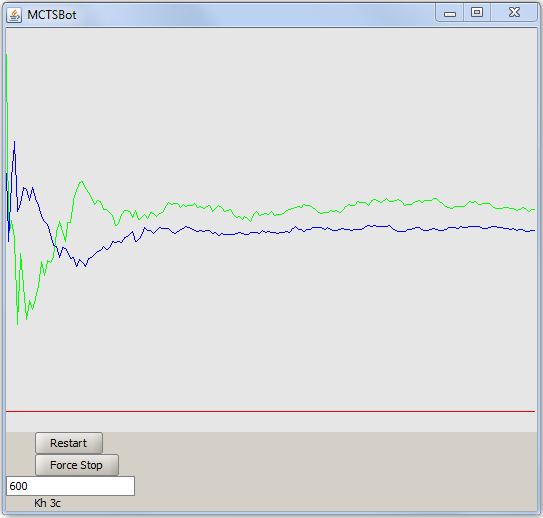
\includegraphics[width=144mm]{Screenshots/GUI.png}
\caption{A GUI for viewing up to date information \\
about the progress of the MCTS algorithm.}
\label{screenshot:gui}
\end{figure}

%TODO: add a screenshot

%So, the GUI was a useful tool in helping me to debug and test the program. It might have been a better idea to implement it earlier in the project than I did (maybe even right at the start) but it still helped me a lot. 



\section{Summary}								% ----

% Review of everything so far.
% Mention the size of the code base. 
% Mention preliminary results.

%Overall, this was a very large project, over 5000 lines of code in total. I'm sure there's probably still a few bugs in it but, as a whole, the program definitely works. From preliminary testing, I have determined that \mbt can usually beat \sbt at a rate of about \$0.20 per game. To put that in perspective, my earliest working version of the program (from Michaelmas term) was losing at about a rate of \$0.25 per game. 

Overall, this was a very large project\footnote{Over 5000 lines of code in total and 58 classes.} and its performance matches my expectations. From preliminary testing, I have determined that \mbt can usually beat \sbt at a rate of about \$0.20 per game. To put that in perspective, my earliest working version of the program (from Michaelmas term) was losing at about a rate of \$0.25 per game. 

In the next chapter, I will evaluate the program much more thoroughly in a variety of situations. 

























